\documentclass[11pt,a4paper]{article}
\usepackage{times,latexsym}
\usepackage{url}
\usepackage[T1]{fontenc}
\usepackage{grffile}

\usepackage{CJKutf8}
\usepackage{fullpage}

\usepackage{tikz-dependency}

\newcommand\BibTeX{B{\sc ib}\TeX}
\newcommand\confname{EMNLP-IJCNLP 2019}
\newcommand\conforg{SIGDAT}

\usepackage{longtable}

\usepackage{amsmath}
\usepackage{tikz-dependency}
\DeclareMathOperator*{\argmax}{arg\,max}
\DeclareMathOperator*{\argmin}{arg\,min}
\DeclareMathOperator{\E}{\mathop{\mathbb{E}}}

\usepackage{amssymb}% http://ctan.org/pkg/amssymb
\usepackage{pifont}% http://ctan.org/pkg/pifont
\newcommand{\cmark}{\ding{51}}%
\newcommand{\xmark}{\ding{55}}%


\newcommand{\Prob}{\mathbb{P}}%

%\usepackage{pslatex}
%\usepackage{latexsym}
\usepackage[english]{babel}
\usepackage[utf8]{inputenc}
\usepackage{bm}
\usepackage{graphicx}
\usepackage{tikz}
\usepackage{xcolor}
\usepackage{url}
%\usepackage[colorinlistoftodos]{todonotes}
\usepackage{rotating}
\usepackage{multirow}



\newcommand{\japanese}[1]{\begin{CJK}{UTF8}{min}#1\end{CJK}}


\usepackage[T1]{fontenc}

\usepackage{pslatex}
%\usepackage{latexsym}
\usepackage[english]{babel}
\usepackage[utf8]{inputenc}
\usepackage{amsmath}
\usepackage{bm}
\usepackage{graphicx}
\usepackage{tikz}
\usepackage{xcolor}
\usepackage{url}
%\usepackage[colorinlistoftodos]{todonotes}
\usepackage{rotating}
%\usepackage{natbib}
\usepackage{amssymb}



\usepackage{natbib}
\bibliographystyle{plainnat}

\usepackage{amsthm}
 

\allowdisplaybreaks

\newcounter{theorem}
\newtheorem{proposition}[theorem]{Proposition}
\newtheorem{corollary}[theorem]{Corollary}
\newtheorem{question}[theorem]{Question}
\newtheorem{example}[theorem]{Example}
\newtheorem{defin}[theorem]{Definition}
\newtheorem{remark}[theorem]{Remark}
\newtheorem{lemma}[theorem]{Lemma}
\newtheorem{thm}[theorem]{Theorem}


\newcommand{\R}[0]{\mathbb{R}}
\newcommand{\Ff}[0]{\mathcal{F}}
%\newcommand{}[1]{\textbf{#1}}


\newcommand{\soft}[1]{}
\newcommand{\nopreview}[1]{}
\newcommand\comment[1]{{\color{red}#1}}
\newcommand\mhahn[1]{{\color{red}(#1)}}

\newcommand{\thetad}[0]{{\theta_d}}
\newcommand{\thetal}[0]{{\theta_{LM}}}
\newcommand{\thetap}[0]{{\theta_{P}}}


\title{Coadaptation between
Usage and Grammar in the Evolution of Word Order across Languages}
% Maybe?: Grammar and Usage Interact in the Evolution of Language

\author{Michael Hahn\\Department of Linguistics, Stanford University\\\\Yang Xu\\ Department of Computer Science, Cognitive Science Program, University of Toronto\\\\ \texttt{mhahn2@stanford.edu}}

\date{}

\begin{document}
\maketitle


\begin{abstract}
Languages vary considerably in syntactic structure.
About 40\% of the world's languages have subject-verb-object order, and about 40\% have subject-object-verb order.
A wide range of existing work has argued that the structure of human language supports efficient communication. In these studies, variation across languages reflects different optima or points along a Pareto frontier. However, the existing theories are not able to explain the  frequency distribution and evolution of word order in individual languages.
We propose a theory of coadaptation between usage and grammar and report evidence for this functional pressure in the evolution of word order across languages. We show in 74 languages from 29 families that they exhibit the basic word order that is most efficient given the sentences typically produced by their speakers, under the joint consideration of grammar for Dependency Length Minimization.
Drawing on phylogenetic modelling and historical text corpora from seven language families, we show that historical word order change is accompanied by change in the usage distributions.
We identify relevant characteristics that reflect this joint optimization, in particular the frequency with which subjects and objects are expressed together for the same verb.
Our findings highlight that functional optimization in language structure and in language usage go hand in hand in shaping the evolution of syntactic structure across languages.
\end{abstract}

%{\color{blue}References}
%This work can be a useful reference (e.g., style of writing, and standard of figures and display items): {\it Cultural influences on word meanings revealed through large-scale semantic alignment}. This work too: {\it The evolution of language families is shaped by the environment beyond neutral drift}. Both papers were published at the same venue, which is suitable for us too if you agree.\\

%{\color{blue}Suggestions and modifications of the outline}\\

%{\color{blue}1. Problem motivation and significance - cross-linguistic variation in syntactic structure, and how it is central to understanding the nature of human language (e.g. Greenberg)}\\

%{\color{blue}2. Existing theory of efficient communication}
%-Introduce efficiency-based explanations

%-Raise variation between languages and what efficiency-based theories have to say about it\\

%{\color{blue}3. Relation of efficient communication and basic word order}

% \cite{greenberg-universals-1963} 



%<<<<<<< overleaf-2020-10-31-0927


%In this

%Here we present evidence that the evolution of syntactic structure reflects an additional functional pressure through coadaptation between the grammatical structure of a language and the way that language is used.


%=======
%>>>>>>> master
% Hawkins 1994, 2004, 2014, Chomsky 2005, Christiansen & Chater2008, Jaeger & Tily 2011, Fedzechkina et al. 2012, Gibson et al. 2019). The idea is thatlanguages are shaped by a trade-off between information transfer and ease
%Human languages show both tremendous variation and striking similarities in their grammatical structure. Understanding these is central to the understanding of the nature of human language.
%A large body of research argues that similarities across languages are due to convergent evolution favoring efficient communication under cognitive resource limitations \citep{haspelmath2008parametric}.
%Here, we present evidence that evolution favoring efficiency jointly affects the grammatical structure of a language and the way the language is used.
%\comment{Try to insert 1 sentence here that says what we study here that differs from or advances the theory of efficient communication, at the end of the opening paragrah.}

%Here, we present evidence that 
%- language use induces change
%Bybee, Complex adaptive system: citing (Perkins 1992, Wray and Grace 2007) t
%% Wray, Allison, and George W. Grace. 2007. The consequences of talking to strangers: evolutionary corollaries of socio-cultural influences on linguistic form. Lingua 117: 543–78.
%cultural factors may play a role in causing typological differences
%- frequent usage patterns come to be reflected in common grammatical patterns
%- grmamatical properties change as language is used
%- locus of change is the way language is used (Chapter 6 of her book). also Croft 2000. other view: transmission is the driver of change Briscoe 2003, Kirby and Christiansen 2003).
%% Croft, William. 2000. Explaining language change. Harlow: Longman Linguistic Library.
%% Briscoe, Ted. 2003. Grammatical assimilation. In M. Christiansen and S. Kirby (eds.), Language evolution, 295–316. Oxford: Oxford University Press.
%- social context affects grammatical structure (Perkins 1992 for deictic distinctions; also Perkins for relative clauses)
%% Perkins, Revere. 1992. Deixis, grammar, and culture. Amsterdam/Philadelphia: John Benjamins.
%- the frequency of constructioin types varies across language (serial verbs [Hopper 2008]),. What is rare in one language may be ungrammatical in another (oblique relative clauses [Keenan 1975];
%% Keenan, Edward L. 1975. Variation in universal grammar. In E. Keenan, R. Fasold and R. Shuy (eds.), Analyzing variation in language, 136–48. Washington, DC: Georgetown University Press.
%% Hopper. 2008. Emergent serialization in English: pragmatics and typology. In J. Good (ed.) Language universals and language change, 253–84. Oxford: Oxford University Press.
%% Hopper. 1984. The discourse basis for lexical categories in universal grammar. Language 60(4): 703–52.
%- Hawkins 
%- what constructions speakers choose to use
%- what is used frequently is coded efficiently (Haspelmath)



The world's languages show considerable variation in syntactic structure \citep{greenberg-universals-1963, baker2001atoms, croft2003typology}.
A large body of research has suggested that this variation is constrained by the functional pressures of efficient communication under limited cognitive resources \citep{haspelmath2008parametric, jaeger2011on, kemp2018semantic, gibson2019how}.
Under this view, the structure of language partly reflects the way that language is used \citep{hopper1984the, bybee1994the, croft2000explaining, bybee2006from} and adapts to optimize  production and comprehension for human communication \citep{hawkins-performance-1994, haspelmath2006against, bybee2010language}.
Here, we draw on large-scale data and phylogenetic modelling to provide evidence that usage and grammar are optimized jointly to maintain efficiency in language change:
Languages tend to be structured efficiently for the utterances that speakers produce, and, conversely, speakers produce utterances that are efficient given the grammar of their language.

A key dimension that languages vary along in syntactic structure is word order.
Typologists have long classified languages according to their basic word order, or the order in which they typically order verbs, subjects, and objects \citep{greenberg-universals-1963}.
About 40\% of the world's languages are classified as following subject-verb-object order ({SVO}, as in English, ``a dog bites a human''), and 40 \% are classified as following subject-object-verb order ({SOV}, ``dog-human-bites'') \citep{wals-81}.
Other orders such as verb-subject-object (``bites-dog-human'') are much less common.
A large proportion of languages has more than one ordering, though typically with one of the orderings being the most common or least marked.
This ordering is considered the  basic word order of a language in the typological literature \citep{greenberg-universals-1963, wals-s6}.


Different theories have been proposed for this word order variation.
The low frequency of object-initial orderings (e.g., OSV) arguably has satisfactory explanations (see below), but there is no consensus on the frequency distribution of SVO and SOV.
Some work has argued that SOV is the default order in the history of language and that SVO has emerged later \citep{givon1979understanding,senghas1997argument, newmeyer2000evolutionary, goldin-meadow2008natural, gibson-noisy-channel-2013}.
On the other hand, phylogenetic modelling suggests that languages can cycle between these two orders in their development \citep{maurits2014tracing}.
Efficiency-based accounts have been argued to either favor SVO or SOV \citep{maurits-why-2010, ferrer-i-cancho-placement-2017}.
\cite{maurits2010why} propose that the frequency of different basic word order pattern is predicted by a tendency to avoid peaks and troughs in the rate at which information is transmitted.
Their model predicts object-initial order to be strongly dispreferred.
However, it also suggests SVO to be considerably more efficient than SOV, even on usage data from an SOV language (Japanese), which contradicts the empirically near-equal frequencies of SVO and SOV.
\cite{ferrer-i-cancho-placement-2017} suggest that SOV and SVO are optimal under different efficiency criteria, but this account does not predict word order on the level of individual languages. 

%Here we show that the efficiency considerations can make fine-grained predictions about word order in individual languages, which crucially depend on language-specific usage patterns.
%Also cite \cite{kemmerer2012cross-linguistic}


We present an alternative account for the frequency distribution of SOV and SVO order and the evolution of word order across languages:
Coadaptation between grammar and usage. We refer to this idea as the coadaptation hypothesis. We propose that neither SVO nor SOV is more efficient in principle.
Rather, languages tend to have the basic word order that is most communicatively efficient given the utterances speakers typically produce.
As languages change, usage and grammar evolve together, such that change in usage goes hand-in-hand with change in basic word order.


The idea that the structure of language is shaped by language use has been discussed in several aspects of language.
For example, it has long been documented that languages provide simpler grammatical coding for categories that are expressed more frequently \citep{greenberg1966language, haspelmath2006against}, and that structures more commonly used in some languages are more likely to be grammatically available in other languages \citep{keenan1975variation}.
It has also been argued that discourse function shapes grammatical catgeories, for instance the noun-verb distinction \citep{hopper1984the} and the coding of grammatical roles \citep{bois1987the}.
\citet{perkins1992deixis} provides evidence that social structure impacts the complexity of deictic inflection across languages; \citet{lupyan2010language} show that languages in small-scale societies tend to have higher inflectional complexity.
\cite{gibson2017color} suggest that color naming systems differ between industrialized and non-industrialized societies due to differences in the usefulness of color in a society, and it has also been argued that the sound systems of languages adapt to climate and diet of the speech community \citep{everett2015climate,blasi2019human}.

%Our study tests this idea using large-scale text data and phylogenetic modeling.


%We extend this idea by hypothesizing that grammatical structure and usage patterns should interact in the evolution of syntax: As a language changes, change in grammatical structure should be accompanied by change in the way the language is used, i.e., there is a process of coadaptation between grammar and usage.

% also Blasi on fricatives, ...
%Efficiency-based accounts of language structure often model optimization for usage distributions that are held constant across languages (CITE).
%Variation between languages is accounted for as reflecting different optima or points along a Pareto frontier \citep{zaslavsky2018efficient, zaslavsky2019evolution}.
%However, in reality, usage patterns do differ between languages, and this might impact which grammatical patterns are more efficient for a given language.

\section*{Theoretical proposal of coadaptation}


Our coadapation hypothesis is grounded in prominent efficiency-based accounts of word order that are centered around various locality principles. These accounts assert that elements are ordered closer together when they are more strongly related in terms of their meaning and function \citep{behaghel1932deutsche,givon1985iconicity,rijkhoff-word-1986,hawkins-performance-1994}.
A classic formalization of this view is Dependency Length Minimization (DLM), the observation that languages tend to order words in such a way as to reduce the overall distance between syntactically related words \citep{rijkhoff-word-1986,hawkins-performance-1994,liu2008dependency,futrell-cross-linguistic-2015, liu-dependency-2017, futrell2020dependency}.
This is supported by corpus studies on dozens of languages, and explains word order universals \citep{rijkhoff-word-1986, hawkins-performance-1994, hahn2020universals}.
Dependency Length Minimization and related locality principles can be justified in terms of parsing efficiency \citep{hawkins-performance-1994}, memory efficiency \citep{gibson-linguistic-1998} and general communicative efficiency \citep{hahn2020universals}.
%Other efficiency principles include Uniform Information Density \cite{...} and noise robustness in transmission \cite{gibson-noisy-channel-2013}.



Our proposal of coadaptation suggests that languages have the basic word orders that are most efficient for DLM, given the utterances typically produced in a language.
To understand how DLM might make fine-grained predictions about basic word order in individual languages, we begin with a thought experiment.
We first consider a simple transitive sentence such as `dogs bite people' (Figure~\ref{fig:sent-dep}A). 
DLM is defined formally in terms of Dependency Grammar~\citep{hays1964dependency,hudson1984word,melcuk1988dependency,corbett1993heads,tesniere2015elements}.
In this formalism, the syntactic structure of a sentence is drawn with directed arcs linking words -- called heads -- to those words that are syntactically subordinate to them -- called dependents.
For instance, arcs link the verb to its subjects and objects.
The length of an arc is one plus the number of other words that it crosses.
The dependency length of an entire sentence is the sum of the lengths of all dependency arcs.

In a simple sentence as in Figure~\ref{fig:sent-dep}, SVO order results in overall lower dependency length:
In SVO order, both dependencies have length $1$, resulting in a total length of $2$.
In SOV order, the arc between the verb and its subject is longer because it crosses the object, resulting in a total length of $3$.
Indeed, based on this consideration, \cite{ferrer-i-cancho-placement-2017} argued that DLM is generally optimized by SVO order, but we will see that the picture is more complex.


\begin{figure}
%\begin{center}
\textbf{A}
\begin{dependency}[theme = simple]
   \begin{deptext}[column sep=1em]
          dogs \& bite \& people  \\
   \end{deptext}
   \depedge{2}{1}{subject (1)}
   \depedge{2}{3}{object (1)}
\end{dependency}
\begin{dependency}[theme = simple]
   \begin{deptext}[column sep=1em]
   \japanese{犬は} \& \japanese{人を} \& \japanese{噛みます}\\ 
   inu-wa \& hito-o \& kamimasu \\
          DOG \& HUMAN \& BITES  \\
   \end{deptext}
   \depedge{3}{1}{subject (2)} %{\parbox{1cm}{subject \\ \\ 2}}}
   \depedge{3}{2}{object (1)}
\end{dependency}

B
\begin{dependency}[theme = simple]
   \begin{deptext}[column sep=1em]
       think \& big dogs \& bite \& people  \\
   \end{deptext}
    \depedge{1}{3}{complement (3)}
   \depedge{3}{2}{subject (1)}
   \depedge{3}{4}{object (1)}
\end{dependency}
\begin{dependency}[theme = simple]
   \begin{deptext}[column sep=1em]
   \japanese{大きな犬が} \& \japanese{人を} \& \japanese{噛むと} \& \japanese{思います}\\ 
   ookina inu-ga \& hito-o \& kamuto \& omoimasu \\
         BIG DOG \& HUMAN \& BITES \& THINK \\
   \end{deptext}
   \depedge{3}{1}{subject (2)}
   \depedge{3}{2}{object (1)}
   \depedge{4}{3}{complement (1)}
\end{dependency}

C
\begin{dependency}[theme = simple]
   \begin{deptext}[column sep=1em]
   \japanese{人を} \& \japanese{噛みます}\\ 
   hito-o \& kamimasu \\
   HUMAN \& BITE  \\
   \end{deptext}
   \depedge{2}{1}{object (1)}
\end{dependency}
\begin{dependency}[theme = simple]
   \begin{deptext}[column sep=1em]
   \japanese{犬は} \& \japanese{噛みます}\\ 
   inu-wa \& kamimasu \\
          DOG \& BITE  \\
   \end{deptext}
   \depedge{2}{1}{subject (1)}
\end{dependency}

        \caption{A: Word order variation across languages. English (left) follows Subject-Verb-Object (SVO) order. Japanese (right) follows Subject-Object-Verb (SOV) order. Such simple sentences where both subjects and objects are expressed tend to favor SVO order. B: Embedded contexts tend to favor SOV order. C: The preference for SVO order is neutralized when only one of the two arguments is expressed. Sentences like these are fully grammatical in Japanese.}
        \label{fig:sent-dep}
\end{figure}

Now consider what happens in more complex sentences, where verbs are embedded as dependents of other words.
In Figure~\ref{fig:sent-dep}B, we consider sentences of the form `I think (that) big dogs bite people'.
Here, dependency length is 5 in SVO order, and 4 in SOV order, reversing the advantage  of SVO order seen in basic sentences.

One might hypothesize that simple unembedded sentences are more frequent than more complex sentences, and that the advantage of SVO in more simple sentences outweighs its disadvantage in embedded contexts.
However, this depends on the precise details of the frequency with which different syntactic configurations appear.
For example, the advantage of SVO in simple sentences is neutralized in sentences where only a subject or only an object is expressed (Figure~\ref{fig:sent-dep}C).
Such sentences, while not always possible in English, are very frequent in languages like Japanese.
Whereas 33 \%  of verbs expressing at least one argument (S or O) in an English corpus express both, only 13 \% do in Japanese (see SI Section X).
This means that the frequency with which different configurations appear in language use influences the degree to which SVO or SOV order are more efficient for DLM.



The reasoning above focused on SVO and SOV, but this approach can be extended to other orderings.
The crucial difference between the two orderings was whether S and O are ordered on the same or on different sides of the verb.
Other orderings can also be classified along this dimension, for instance, VSO as the third-most ordering patterns with SOV with respect to Figures \ref{fig:sent-dep} A--C.

Note that DLM does not make predictions as to the direction in which subject and object should appear. Since the length of dependencies does not depend on their direction, there is no difference between, say, SOV and VOS.
Independent principles are needed to explain why SOV and SVO are more common than, say, VOS and OVS.
A key component is a strong preference for subjects to come earlier \citep{wals-81}.
Subjects often are animate and given in prior discourse, and phrases with these properties generally tend to go earlier in sentences across languages \citep{prince1981toward, mcdonald1993word}.
This principle favors, say, SVO over OVS, while being equally well satisfied by SVO and SOV order.

Here we provide evidence that languages show coadaptation between their basic word order and the frequencies with which different syntactic configurations are used.
Specifically, we contrast orderings that order S and O on the same or different sides of the verb. We test the coadaptation hypothesis using data from over 70 languages by computing, for each language, which basic word order is most efficient given its usage distribution as recorded in large-scale text corpora. We then use a model of drift on phylogenetic trees to assess whether languages have evolved historically toward states where usage distributions and actual basic word order are aligned.



%Now explain examples from presentations, in particular how frequency of co-expression of S and O can differentially favor SVO or SOV. {\color{blue} this is good -- i wonder if you want to illustrate the throught experiment or the basic idea of coadaptation in an opening diagram.}\\




%\comment{at the end of the intro, it might benefit to provide a preview or plan for the rest of the paper, i.e. you could say how we plan to test the coadaptation hypothesis in x, y, z, ways, so that the later studies can be pre-empted here so as not to be very surprising.}

%{\color{blue}4. related to the above paragraph -- state limitations of existing theory/approach and our proposal. Articulate how existing theories of efficient communication may be limited or insufficient to explain basic word order variation across languages, and change over time. Therefore introduce the new proposal of coadaptation. (also, if we stick with ``coadaptation'', then don't use ``co-adaptation'') }

%\mhahn{TODO fix this}

%existing proposals insufficient:



%Existing efficiency-based theories of word order variation:






%http://tedlab.mit.edu/tedlab_website/researchpapers/Gibson_et_al_2013_PsychSci.pdf

%- our results argue against work that has suggested SVO as the more efficient order (Gibson et al 2013, \url{https://www.ncbi.nlm.nih.gov/pmc/articles/PMC4534792/})

%\url{https://www.eva.mpg.de/fileadmin/content_files/linguistics/conferences/2015-diversity-linguistics/Hammarstroem_slides.pdf}

%- Trudgill,2011

%- Gell-MannandRuhlen2011,MauritsandGriths2014

%\section{Study 1: Evidence for Coadaptation}
\section*{Results}

\subsection*{Cross-linguistic Evidence for Coadaptation}

We begin by testing whether basic word order reflects coadaptation across different languages.
%We test the  hypotheses: Basic word order reflects coadaptation between grammar and usage (\textsc{Coadaptation}), basic word orders differ in their efficiency for DLM as proposed by \citep{ferrer-i-cancho-placement-2017} (\textsc{DifferentEfficiencies}), or there is no crosslinguistic relation between .
If there is coadaptation between basic word order and usage, we expect that languages should have the basic word order that is most efficient given their usage distributions.
Alternatively, we expect that, either, one of the two basic word orders is systematically more efficient for DLM, or there is no systematic relationship between basic word order and dependency length.


%First, we first use the label from WALS, which we partitioned into different-side, same-side, and free.
%Second, as a rough measure (CITE), corpus-based, whether O and S have the most-frequent direction in the treebank.


We compare two groups of word orders: SVO-like order where S and O are ordered on different sides of the verb, and SOV/VSO-like order where S and O are ordered on the same side of the verb.
Languages can fall on a spectrum between languages with entirely strict SVO order and languages with entirely strict SOV order~\citep{steele1978word}.
English is close to one end of the spectrum with dominant SVO order, with rare exceptions (e.g., stylistically marked VS order in ``then came a dog'').
Japanese falls entirely on one end of the spectrum, allowing only SOV and OSV order.
Many languages occupy intermediate positions. 
For instance, in Russian, all logically possible orderings of S, V, O can occur, though with different frequencies.

We quantify the position of an individual language on this continuum using a quantitative corpus-based metric which we refer to as subject-object position congruence.
This metric indicates the chance that two randomly selected instances of S and O from a corpus -- not necessarily from the same sentence -- are on the same side of their respective verbs. This number is 1 in strict SOV languages like Japanese, close to 0.5 in languages with flexible word order, and close to 0 in English.

%We propose two quantitative metrics measuring where a language falls on this spectrum.
%First, we count how often S and O appear on the same side of a verb that realizes both S and O arguments ({Same-Side Count}).\mhahn{Are there better names for these measures?}
%This measure does not take into account what happens in sentences where only S or O is realized.


We compare these measures between observed word orders and hypothetical orderings obtained by optimizing for Dependency Length Minimization. We approximate the distribution over different syntactic configurations using large corpora.
We draw on the Universal Dependencies data, which includes text data annotated with syntactic tree topologies from over 70 languages from 29 language families (\citep{zeman2020universal}, see Methods for details).
For each language, we construct orderings that are approximately optimized for DLM.

To parameterize the approximately optimized orderings, we adopt the established model of counterfactural order grammar introduced by \citet{gildea-optimizing-2007}.
These are simple, parametric models parameterizing how the words in a syntactic structure are linearized depending on their syntactic relations.
For instance, such a grammar may specify that subjects follow or precede verbs, and that adjectival modifiers follow or precede nouns (see Methods for details).
We use the method in \citet{hahn2020universals} to construct grammars that approximately minimize average dependency length using stochastic gradient descent.

In order to control for variation across different optima, for each of the 74 languages, we construct 15 approximately optimized grammars, and compute the average subject-object position congruence across these counterfactual orderings.

%\comment{** to what extent we can justify that our approach is not somewhat circular? in particular, the optimized grammars were derived from the corpora, which were used to determine the empirical frequency proportions of the basic word order -- i think some statements are needed here to suggest that there's some independence between the optimized grammar predictions by the model, and the empirical distributions.}

%\comment{** Do you plan to say a bit more details about 1) the conterfactual order grammar, and 2) the data, 72 languages, where they came from, and why they are a reasonable sample, either in Methods, and/or in Appendix? I think these details would be needed for reproducibility but also for careful description of the materials and methods. also, you should say how many language families are covered in the 72. languages.}

Under our coadaptation hypothesis, we expect that the subject-object position congruence of optimized orderings should correlate with a language's actual subject-object position congruence.
Otherwise, if one order is more efficient in principle, or there is no systematic association between basic word order and DLM, then no such correlation should be seen.


While the optimized grammars and the attested orders are computed on the basis of the same corpus data, the optimized grammars are derived entirely and independently from the tree topologies, and the original word orders are not involved in their calculation (See SI Section 9 showing that results hold similarly when estimating optimized grammars and attested orders using disjoint subsets of corpora).



In Figure~\ref{fig:study1}A, we visualize real subject-object symmetries against the average subject-object position congruence in the 74 languages.
Without controlling for dependencies between related languages, model-predicted and attested subject-object position congruence are correlated ($R=0.49$, $p<10^{-5}$).
In order to account for the statistical dependencies between related languages more rigorously, we conducted a regression where we entered language families as random effects with random slopes and intercepts.
Attested subject-object position congruence was strongly predictive of subject-object position congruence in the optimized grammars ($\beta = 0.44$, $SE=0.11$, $95\%$ credible interval $[0.24, 0.66]$, $P(\beta<0) < 10^{-4}$).
This result provides strong support for the coadaptation hypothesis: Languages tend to have the basic word order that is most efficient given their tree structure distributions.
It is incompatible with the suggestion that SVO is generally more efficient (than SOV) for DLM \citep{ferrer-i-cancho-placement-2017}.



%It is incompatible with the \textsc{MultipleOptima} or \textsc{NoOptimization} hypotheses.

%\comment{should say a few more details, e.g. why you chose a mixed effect model, for instance, you could say in order to control for x, y, z, we performed a mixed-effect ...}

%\comment{Somewhere in introduction, we should probably single out a paragraph and make it explicit the idea of the "coadaptation hypothesis: xyz....", so that we can keep referring to that phrase later in results.}

%{\color{blue} If you plan to go for NHB, then you can encapsulate some methodologies in the Methods section and focus on explaining and interpreting the main results.}


\begin{figure}
    \centering
    A
    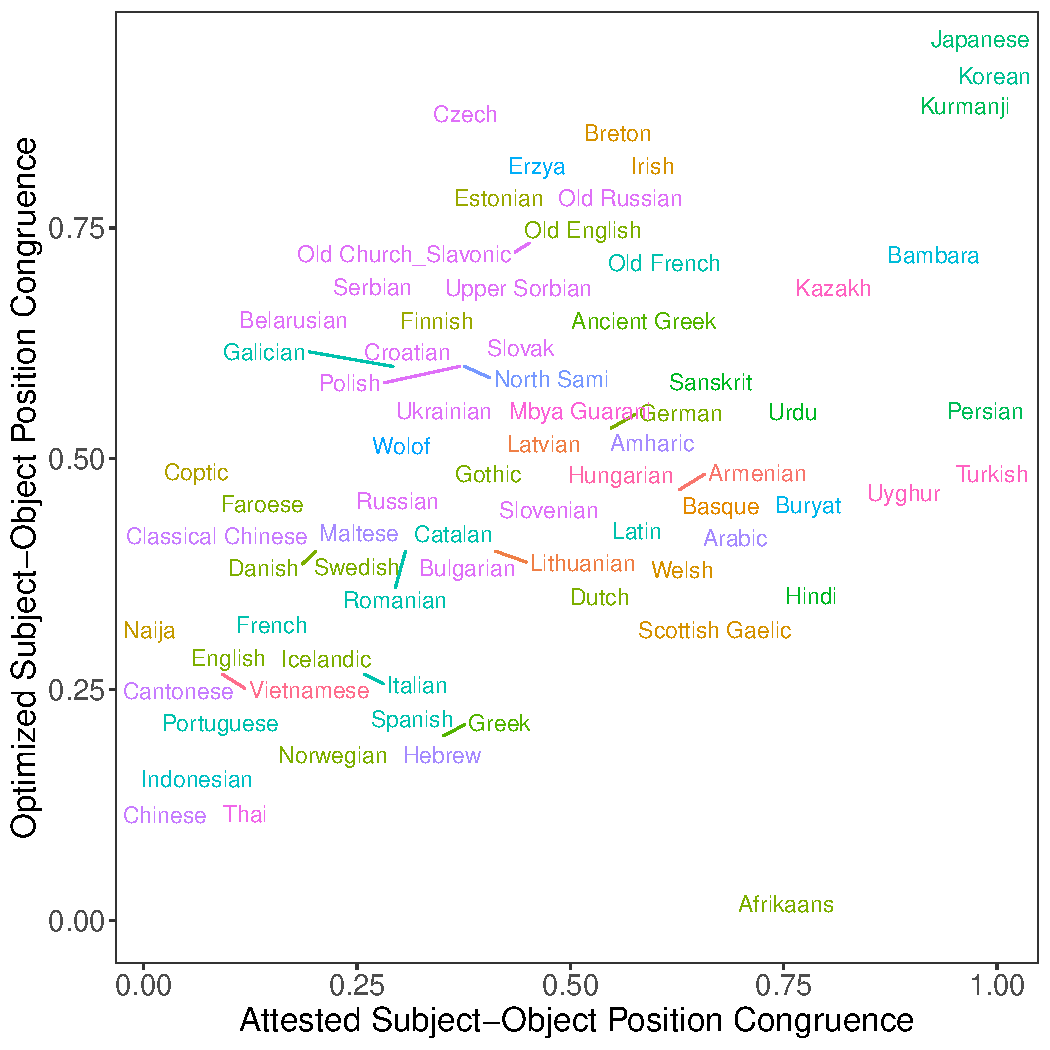
\includegraphics[width=0.46\textwidth]{../analysis/figures/fracion-optimized_DLM_2.6_format.pdf}
    B
    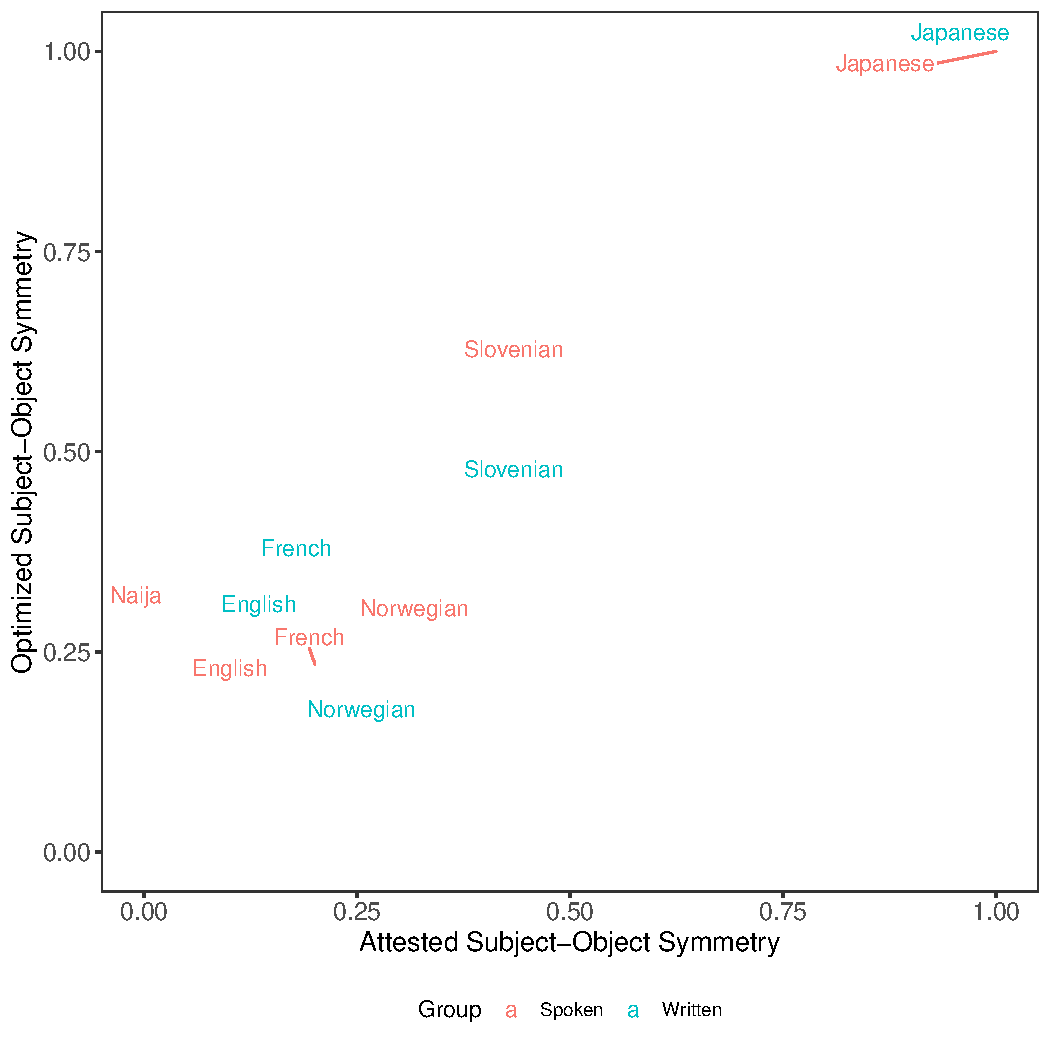
\includegraphics[width=0.46\textwidth]{../analysis/analysis_spoken/spoken.pdf}
    \caption{Evaluation of the coadaptation hypothesis across languages. a) subject-object position congruence in attested (x-axis) and approximately optimized (y-axis) orderings. Languages are colored by language families. Small lines connect labels to the position of the language, where needed to avoid overlapping labels. b) Comparison of subject-object position congruence between written (blue) and spoken (red) corpora in six languages where spoken corpora are available. Note that, for one language (Naija), all available data is in spoken form.}
    \label{fig:study1}\label{fig:spoken}
\end{figure}


%\section{Analysis 2: Spoken Corpora}

%\comment{maybe somewhere here or nearby you should acknolwedge that there are only very limited number spoken corpora available, but nevertheless we found these and suggest that these languages span the spectrum of word order variation.}


We have approximated the usage distribution over syntactic configurations using (written) text corpora.
Although the vast majority of existing annotated corpus data is in written form (e.g., news and web text), spoken language is thought to be most important for language change, particularly since widespread literacy is very recent.
We therefore collected all spoken corpora in dependency format that we could obtain access to, resulting in data from six languages (see Methods), and verified whether the conclusion of our cross-linguistic analysis holds on data from these spoken-language treebanks. Figure~\ref{fig:spoken}B
shows results on these treebanks and the comparison to written data from the same languages.
There is a strong agreement between written and spoken data from the languages we analyzed. Specifically, there are strong and significant correlations between real and predicted subject-object position congruence in both written ($R=0.96$, $p=0.0023$) and spoken ($R=0.94$, $p=0.0048$) data, in agreement with the coadaptation hypothesis.
%In a linear regression with subject-object position congruence among optimized grammars as the dependent variable,  ($\beta=1.11$, $SE=0.29$, $95\%$ CrI $[0.58, 1.69]$).\footnote{The small number of datapoints does not support a mixed-effects analysis. Even with strong priors and more iterations, we encountered small values of Tail Effective Sample Size. However, we found qualitatively similar results when excluding either English or Norwegian, in which case all languages come from different families, and the simple linear model is fully appropriate.}.
%This result is in agreement with that from the full set of corpora.
%\mhahn{TODO the other measure}
%\mhahn{what is the dependent and independent variables in the linear regression? (and perhaps why a Bayes LR as opposed to a plain LR? need to justify a bit more}



%\section{Analysis 2: Historical Evolution}


%We also drew on languages where dependency treebanks with data from different stages of the same language are available (see Materials and Methods for details).

%We also drew on languages where dependency treebanks with data from different stages of the same language are available (see Materials and Methods for details).

%The diagonal in Figure~\ref{fig:study1} describes those points where usage and grammar match perfectly in basic word order, i.e., those points where the real order distribution is identical to the order distribution among optimized grammars, given the distribution over tree topologies.
%Therefore, if the coadaptation hypothesis is true, then languages should stay close to or move towards the diagonal in the plane described by predicted and real subject-object position congruence.

\subsection*{Evolutionary Evidence for Coadaptation}
We have provided evidence for the coadaptation hypothesis using a cross-sectional analysis of 74 contemporary languages.
If variation in word order reflects coadapation between grammar and usage, we should expect to see coevolution of basic word order and usage as languages evolve over time.
To test this proposal, we conducted a phylogenetic analysis on the evolution of usage and word order.
Phylogenetic analyses have previously been applied to studying the historical evolution of languages~\citep[e.g., ][]{gray2009language,greenhill2009austronesian,chang2015ancestry,sagart2019dated}, including the evolution of word order patterns \citep{dunn-evolved-2011, maurits2014tracing}.


A phylogenetic analysis allows us to construct an explicit model of language change, drawing on two sources of information:
First, in several cases, our dataset includes data from different stages of the same language (such as Ancient Greek and Modern Greek).
Such datasets provide direct evidence of diachronic development.
Second, using phylogenetic information, the model can also draw strength from contemporary language data:
Data from related languages may permit inferences about their (undocumented) common ancestor, and thus about possible trajectories of historical change \citep{pagel2004bayesian, dunn-evolved-2011, maurits2014tracing}.


We used a model of random walks on phylogenetic trees \citep{felsenstein1973maximum,pagel1997inferring, pagel2004bayesian} to model how grammar and usage of a language evolve over time, in order to test the coadaptation hypothesis over history.
We describe the state of a language $L$ at time $t$ as a vector $\xi_{L,t} = (X_{L,t}, Y_{L,t})$ in the plane spanned by usage (optimal subject-object position congruence) and grammar (real subject-object position congruence).
Whenever a language splits into daughter languages, the point $\xi_{L,t}$ continues to evolve independently in each daughter language.
As the components of $\xi_{L,t}$ are continuous, we model their change over time using a random walk given by an Ornstein-Uhlenbeck process (\citep{felsenstein1988phylogenies,hansen1997stabilizing, blackwell2003bayesian}, see Methods for details).
This process is parameterized by rates of change in the two dimensions and the correlation between the changes in both dimensions \citep{felsenstein1973maximum,hansen1997stabilizing, freckleton2012fast}.
Under the coadaptation hypothesis, changes in both dimensions should be positively correlated.
Under the null hypothesis, no such correlation should be expected.
Besides rates of change, the model also incorporates the possibility of a bias towards specific regions of parameter space (e.g., low or high subject-object position congruence).

We obtained phylogenetic trees for the 74 languages in our sample (see Methods), and inserted historical stages as inner nodes in these trees.
We fitted the parameters of the model using Hamiltonian Monte Carlo methods (see Methods for details).


%First, for several languages, corpus data from different stages is available.
%For example, there are dependency treebanks both of contemporary English and Old English (approx. 900 AD).
%There are also cases where data is available from the ancestor of several contemporary languages (e.g., Latin is the ancestor of seven languages in our dataset).


%We obtained phylogenferenvnetic trees for the languages in our dataset (see Materials and Methods for details).
%We modified these trees by adding historical stages of existing languages for which we have corpora, such as Old English (approx. 900 AD) as an ancestor of English.



We visualize the resulting model fit in Figure~\ref{fig:drift-model}.
The blue distribution indicates the stationary distribution of the process, i.e., after long-term evolution, a language will tend to be lie within this distribution.
For illustration, we also illustrate the predicted direction of future changes in four languages in red (English, Russian, Arabic, Japanese).

According to the model, changes in grammar and usage are positively correlated:
This is reflected both in the short-term directions of change, which concentrate along the diagonal direction, and in the stationary distribution, according to which languages come to concentrate around the diagonal.
In the stationary distribution, the positions that languages occupy along the two dimensions are strongly correlated ($R=0.73$, $95\%$ credible interval $[0.28, 0.96]$).
Model fit was considerably worse in a lesioned model where the correlation between changes in both direction was constrained to be zero (estimated Bayes Factor: 232).


\begin{figure}
    \centering
    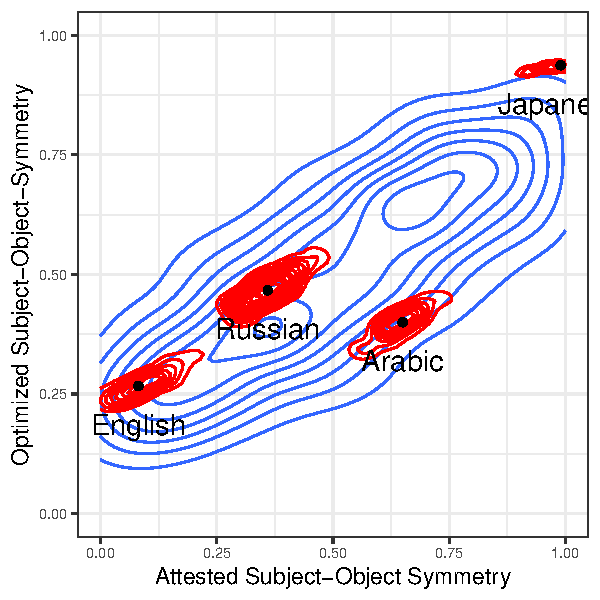
\includegraphics[width=0.5\textwidth]{../change/visualize/stationary.pdf}
    \caption{Result of the phylogenetic drift analysis.
    The blue distribution indicates the estimated long-term stationary distribution of languages, indicating where languages tend to lie after long-term evolution.
    The red distributions indicate predicted states for four individual languages over the next 100 years. Languages are predicted to show co-evolution along grammar (x-axis)  and usage (y-axis).}
    \label{fig:drift-model}
\end{figure}

%\begin{figure}
%    \centering
%    \includegraphics[width=0.5\textwidth]{TODO}
%    \caption{The phylogenetic tree used in our analysis.}
%    \label{fig:phylogenetic-tree}
%\end{figure}


We visualize the evolution of languages where multiple historical stages are documented in Figure~\ref{fig:historical}.
The sample includes multiple languages that started with flexible order and moved towards SVO (English, Romance, East Slavic and Eastern South Slavic, Greek), languages that have remained SVO (Chinese), and languages that have remained predominantly SOV (Indo-Aryan).
% for English
% for Romance
% for East Slavic
% for Eastern South Slavic
% for Greek: \citet{taylor1994change}
% for Chinese
% for Indo-Aryan

In languages that have remained SVO (Chinese), predicted subject-object position congruence moved towards its true values; that is, these languages appear to have evolved their usage patterns in a way that makes their basic word order more efficient.
The two Indo-Aryan languages in our sample, which have remained predominantly SOV, show little movement in either dimension, slightly away from the diagonal.
Finally, among the remaining languages, which started with flexible order and moved towards SVO, all moved along or towards the diagonal.

%\mhahn{is there a way to also quantify this result?}
%\comment{** yes it might be desirable and even necessary to quantify these results -- is there any alignment metric we can use to determine how well the historical shift aligns with the diagonal, or S-O Position Congruence reference points? and then compare that alignment metric to some chance value, e.g. by shuffling data across time or era---use this as a null distribution; then report the p-value of the observed, non-shuffled cases? you can then juxtapose the null trajectories (mean + confidence band, in very light color) on the plot to show people how the real trajectory of historical change deviates from the null.}

%We compare to counterfactual trajectories where
%- languages changed only in usage or in order
%- we 

While our sample includes historical languages that later shifted towards SVO (low subject-object position congruence), it does not include historical languages that later shifted towards SOV (high subject-object position congruence).
The model (and the coadaptation hypothesis) predicts that a language that changed towards SOV should have correspondingly moved towards the top-right of the plane. 
Currently, no annotated treebanks are available for such a language to directly test this prediction; our prediction can be tested once such a treebank becomes available.
We observe that our model indicates no evidence that languages tend to drift towards either SOV or SVO in the long run.
This is shown by the fact that the long-term stationary distribution is equally spread across both low and high subject-object position congruence.
A lesioned version of our model that explicitly prohibits a bias in development provided essentially identical model fit (estimated Bayes Factor 1.1).


\begin{figure}
    \centering
    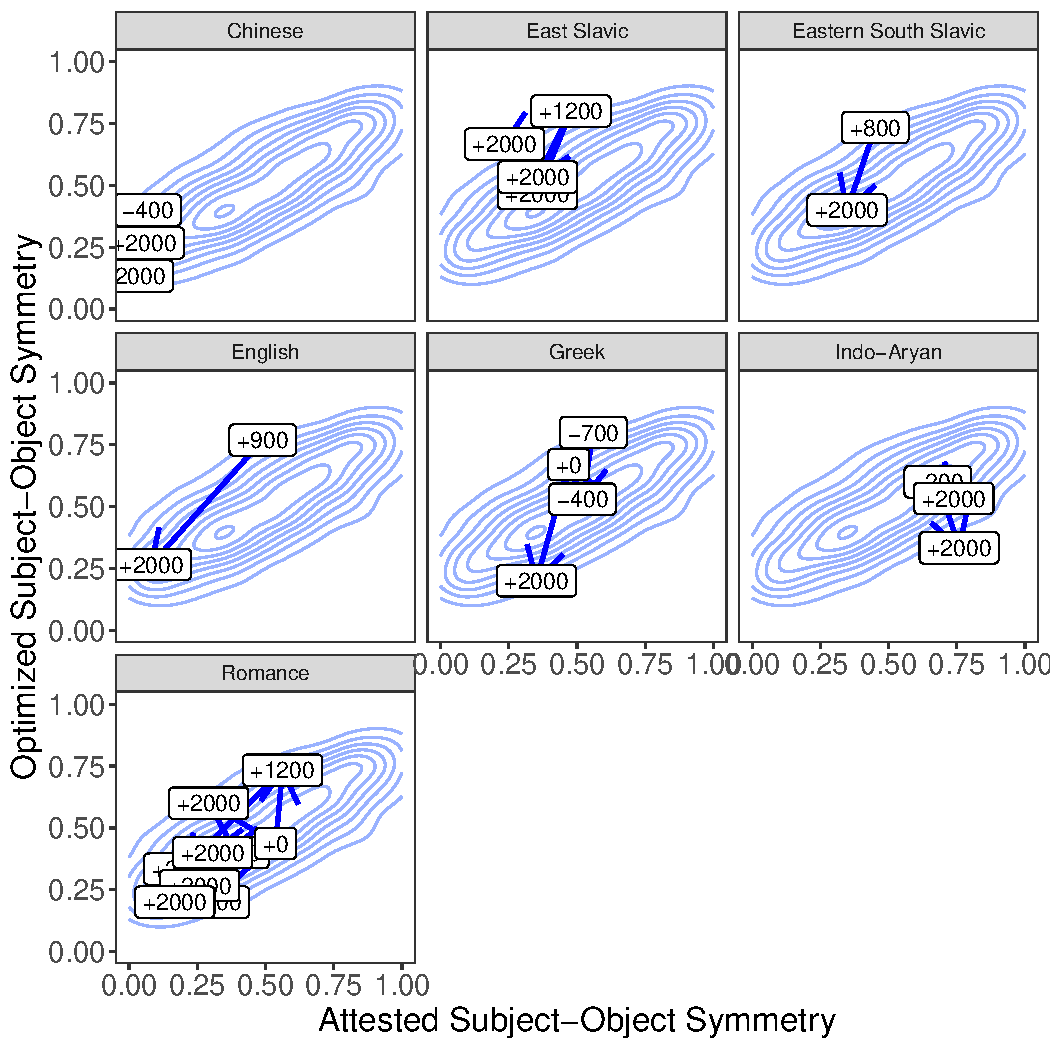
\includegraphics[width=0.95\textwidth]{../analysis/figures/historical_2.6_times_stationary.pdf}
    \caption{The evolutionary trajectories of seven languages or language families with documented ancestors. For each point in the trajectories, we indicate an approximate date. The blue background distribution indicates the long-term stationary distribution of all languages combined according to the phylogenetic analysis. }
    \label{fig:historical}
\end{figure}

Unlike the conventional classification of languages into discrete basic word order categories such as SVO and SOV, the notion of subject-object position congruence accounts for the well-known fact that languages differ in their degrees of word order flexibility \citep{steele1978word}.
To evaluate whether this notion provides a more fine-grained account of word order evolution than the standard classification, we evaluated whether optimized subject-object position congruence predicts attested subject-object position congruence beyond the level of discrete word order categories.
We labeled the languages in our dataset for discrete word order categories (``SVO'', ``SOV'', and rarer categories ``VSO'', ``No dominant order'') based on \citet{wals-81}, supplemented with data from \citet{gell-mann-origin-2011} (see SI Section 6 for details).
First, we found that attested and optimized subject-object position congruence were correlated even within categories ($R = 0.52, p = 0.0002$ within SVO, $R=0.45, p=0.07$ within SOV). 
Second, we conducted a version of the phylogenetic analysis that evaluates whether coadaptation happens beyond the level of these discrete basic word order categories.
We did this by allowing the term that encodes bias to specific regions of parameter space to vary with the basic word order category  (see Methods for details).
The model continued to predict a positive correlation between changes in the two dimensions ($R=0.53$, $95\%$ credible interval $[0.22, 0.78]$, $Pr(R < 0) = 0.00075$).
This shows that the coadaptation hypothesis predicts basic word order at a more fine-grained level than the standard categorical classification, by predicting the frequency of different orders within individual languages.


A well-known variable covarying with word order is case marking: Languages with case marking are more likely to have free word order, and loss of case marking has been argued to correlate with word order becoming more fixed or shifting towards SVO \citep{vennemann1974explanation}, and, conversely, SOV languages mostly have case marking \citep[Universal 41]{greenberg-universals-1963}.
This has a clear functional motivation, because case marking can distinguish subjects and objects when order does not.
In our sample of historical trajectories, movement towards low subject-object position congruence coincides with the loss of case marking in some cases (English, most of Romance, East South Slavic), whereas other languages changed while preserving their case marking systems (Greek \citep{taylor1994change} and East Slavic \citep[p. 242--4]{matthews1960russian}).
This raises the question whether our results can be explained away by assuming that both grammar and usage change in response to changes in case marking.
We found that the phylogenetic analysis continued to predict co-evolution between usage and word order even when controlling for the presence or absence of case, with essentially no change in the predicted strength of correlation (see SI Section 7.1).
This indicates that languages exhibit coadaptation between word order and usage patterns beyond what is captured by the presence or absence of case marking.

%The model provides no evidence that language evolution favors high or low subject-object %aPosition Congruence.
%Visually, the stationary distribution in Figure~\ref{fig:drift-model} is essentially centered with equal weight given to low and high real subject-object position congruence.
%a lesioned model explicitly enforcing absence of such a bias provided essentially identical model fit (Bayes Factor TODO).
%While this conclusion is based on our sample of 74 languages for which dependency treebanks are available, it agrees with the results of \citep{maurits2014tracing} based on a larger sample of languages (albeit from a smaller number of families).





%\section{Analysis 3: Co-Expression of Subjects and Objects}

%\mhahn{TODO I'll still expand this section}
%\comment{description here seems a bit brief; elaborate more? or say in what way is this result interesting, or surprising, or novel (to the literature)?}


\subsection*{Influence of Usage on Word Order}
So far, our results provide evidence for coadaptation between usage and basic word order in the evolution of language.
In what aspects of usage patterns do languages vary and change that reflect this coadaptation?
That is, in what ways do usage patterns influence which basic word order is optimally efficient?
We hypothesize that languages favor SOV-like orders more when they do not frequently coexpress subjects and objects on a single verb.
Indeed, it has been argued, based on evidence from Turkish and Japanese, that SOV languages omit arguments or use intransitive structures more frequently than SVO languages do \citep{hiranuma1999syntactic,ueno2009does,luk2014investigating}, though this might not hold for Basque \citep{pastor2013processing}.
We tested this idea on a larger scale using the corpora in our sample.
We quantified the frequency of co-expression of subjects and objects by calculating what fraction of all verbs that realize at least a subject or an object simultaneously realize both.
We show this ratio together with attested subject-object position congruence in Figure~\ref{fig:study2}.
In a linear mixed-effects models, with by-family intercept and slope, attested subject-object position congruence was predictive of this fraction ($\beta=-0.11$, $SE=0.05$, $95\%$ credible interval $[-0.21, -0.01]$).
Optimized subject-object position congruence was also predictive of this fraction ($\beta=-0.13$, $SE=0.06$, $95\%$ credible interval $[-0.24,  -0.02]$).
%These results were not accounted for by differences in the grammatical availability of unexpressed pronominal subjects (\textit{pro drop}, see SI Section 7.2).
This shows that languages differ in the rate at which they coexpress subjects and objects, and that this is a factor through which usage statistics can influence word order.
We also found such an association between order and coexpression within individual languages: Languages with word order flexibility tend to order subjects differentially depending on the presence or absence of an object, in a way consistent with DLM (see SI Section 8).



\begin{figure}
    \centering
    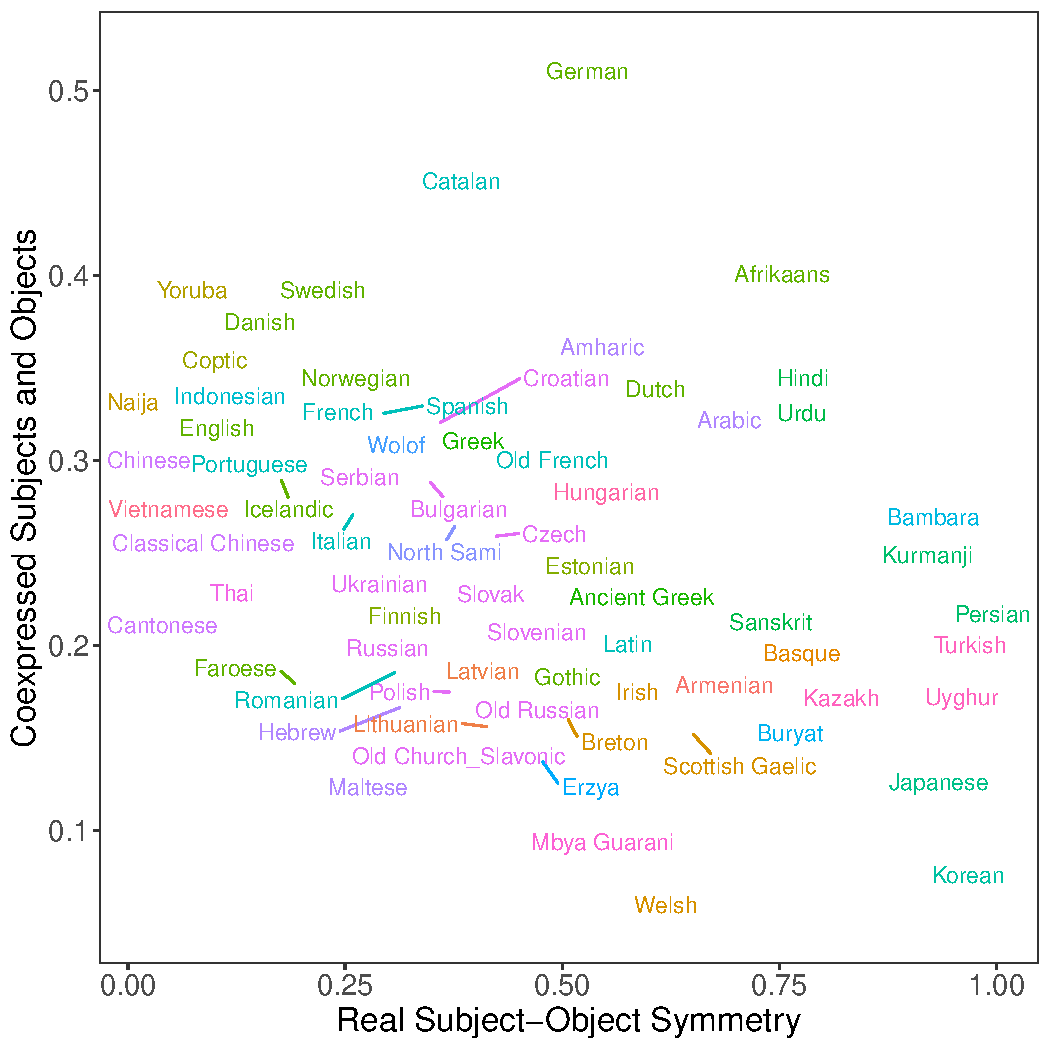
\includegraphics[width=0.7\textwidth]{../analysis/figures/objects-order-pureud-byVerb_FORMAT.pdf}
    \caption{Comparison of attested subject-object position congruence (x-axis) and the fraction of verbs that simultaneously express a subject and an object (y-axis).}
    \label{fig:study2}
\end{figure}




%We also find evidence for a relation between order and co-expression within individual languages, i.e., languages choose different word orders  (see SI Section X). %In many languages, subjects of intransitive verbs -- verbs which do not take an object -- can sometimes appear after the verb (e.g., ``along came a dog'', see SI Section X).
%This provides evidence that, when languages show variation between different word order patterns, the choice of word order for a sentence helps optimize for DLM.
%Within languages, we found that individual sentences tend to have the basic word order that optimizes DLM (see SI Section XX).



%VSO favors agreement, SOV favors case marking. But SOV also have verb agreement a lot, might help zero anaphora






%We do not find evidence between order and the frequency of embedding on the between-language level (TODO), but there is evidence within languages.
%In some predominant VSO languages, SVO is an alternative word order in unembedded clauses (e.g., Standard Arabic, Berber, Ancient Egyptian, see SI Section X).
%Conversely, in some SVO languages, embedded clauses may show VSO order (Bantu, see SI Section X).




%Say something specific:
%Furthermore, we specifically considered what distinguishes the tree topologies of Old English from those of Modern English.
%- Old English -- English what distinguishes the tree structures?
%In this respect, Old English patterned more like contemporary Japanese.




%- Continental West Germanic (except Yiddish). Main clauses predominant SVO/OSV; embedded clauses SOV/OSV.
%- languages with predominant VSO, but alternative SVO in matrix clauses: Standard Arabic, Berber, Ancient Egyptian
%- relative clauses in Bantu: Demuth,Katherine,andCarolynHarford.1999.Verb raising and subject inversion in Bantu relatives. Journal of African Languages and Lingustics20:41ñ61.


%\section{Discussion}


%{\color{blue} 1. how this work impacts the research on basic word order, and particularly, extends the theory of efficient communication and suggests new functional pressures in shaping the evolution of syntactic structure.}\\

%{\color{blue} 2. how this work is limited.}

\section*{Discussion}

We have investigated the frequency distribution and historical change of word order  across languages and found that usage and basic word order interact intimately in their evolution,  which reflects a process of coadaptation  between usage and grammar.



%Our results do not speak to the causal direction of changes in individual languages: 
%While, in a given language, a change might first appear in one aspect (e.g., language use), the preservation of efficiency can lead to compensating changes in another aspect (e.g., grammar).
%Consequently, grammar and usage constrain each other in the process of evolution.
%In the future, the availability of historical data with higher temporal resolution might make it possible to also trace the causal direction of change in individual languages.


%The theory of coadaptation provides a fine-grained account for the distribution of basic word order.
%Going beyond existing accounts of word order, it 


Our results go beyond existing efficiency-based accounts of word order by making specific predictions for individual languages based on their usage distributions.
The model of \cite{maurits2010why} accounts for the low frequency of O-initial orders, but it underpredicts SOV and predicts SVO as the most efficient order even when it is applied to Japanese (i.e., an exemplary language for SOV order).
In comparison, our account explains the language-dependence of basic word order.
For Japanese, DLM correctly predicts S and O to be on the same side of the verb (Figure~\ref{fig:sent-dep}), in contrast with the model of \cite{maurits2010why} that predicts SVO across languages. % {\color{red} that predicts differently how, say more?}.
%\citet{ferrer-i-cancho-placement-2017} argues that SVO and SOV are favored by DLM and predictability maximization, respectively; our work shows how in fact the distribution of basic word orders across languages can be derived from DLM, given the usage distributions. {\color{red} say a bit more -- so what?}.

It has been argued that there is an inherent directionality in the evolution of basic word order, and that SOV is the default or original order in the history of language.
Many historically documented word order changes have gone from SVO to SOV, and the protolanguages of several extant families are thought to have been SOV \citep{givon1979understanding, newmeyer2000evolutionary, maurits2014tracing}.
However, only a small fraction of all word order changes are directly documented through written evidence of historical languages.
\cite{maurits2014tracing}, using phylogenetic modelling, found that languages can cycle between SOV and SVO over long-term development, with little bias towards either order.
The strongest evidence that SOV might be the `default' order comes from recently emerged sign languages \citep{senghas1997argument, sandler2005emergence, goldin-meadow1998spontaneous, meir2010emerging} and from gesturing tasks \citep{goldin-meadow2008natural, langus2010cognitive}.
The theory of coadaptation predicts that new emerging languages tend to have tree structures that favor SOV order.
Indeed, multiple studies report high frequencies of utterances where only one argument is expressed in recently emerged sign languages and homesign systems (\citet{sandler2005emergence} \citet{goldin-meadow1998spontaneous}\citep[p. 31]{neveu2016sign}\citep[p. 622]{ergin2018development}), and in sign languages more generally \citep{napoli2014order}.
% also this dissertation on homesign  also senghas report one-argument uitterances
%Adopting the view that SOV is the historically earlier order, \citet{gibson-noisy-channel-2013} argue that SVO arises as a strategy to reduce ambiguity in the absence of case marking.
%However, the availability of case marking alone is not sufficient to explain the distribution of word order patterns; our results show that coadaptation is present even when controlling for the presence of case marking (see SI Section X) {\color{red} so how did our work advance or impact Gibson et al's work? say a bit more}.


Assuming that SOV is the historically earlier order, some studies have further argued that SVO order later arises to avoid ambiguity in communicating reversible events \citep{gibson-noisy-channel-2013, hall2013cognitive}, to communicate more complex structures \citep{langus2010cognitive, marno2015a, ferrer-i-cancho-placement-2017} and intensional predicates \citep{schouwstra-semantic-2011,napoli2017influence}, or to reduce dependency lengths~\citep{ferrer-i-cancho-placement-2017}.
Under this view, the distribution of SOV and SVO arises from a tension between distinct cognitive and communicative pressures favoring SOV and SVO, respectively~\citep{langus2010cognitive}.
However, this view does not explain the fine-grained per-language distribution of word order patterns, as it does not explain why specific languages have SVO or SOV order.
The theory of coadaptation provides a more precise account of the fine-grained distribution in two ways. First, it explicitly accounts for the language-dependence of word order, providing per-language predictions of optimal word orders.
Second, unlike accounts in terms of a categorical SVO/SOV distinction, it predicts language-specific frequencies of SVO- and SOV-like orderings within individual languages.


%gesture:
%\citep{marno2015a}: availability of lexicon and more elaborate syntactic structures favors SVO
%\citep{langus2010cognitive} SOV emerges in improvised communication, but the compitational system of grammar prefers SVO
%reversible events in gesture \citep{hall2013cognitive}
%\citep{schouwstra2011semantic}: intensional events favor SVO
% TODO cite this? hhttps://www.frontiersin.org/articles/10.3389/fpsyg.2015.01183/full



% Sandler et al
% SV 58
% OV 55
%OIV 1
% VO 13

% SOV 19
% SIOV 3
% SOIV 1
% SVO 6
% SVIO 2
% SOVI 1


%On the prevalence of word orders:
%- roughly equal, e.g. Tomlin 1986

%- theory predicts languages to evolve to SVO unless they have case marking

%claim of correlation between case marking and SOV: Greenberg, 1963; Venneman, 1973; Dryer, 2002; Croft, 2002 (but VSO doesn't seem to favor case so much)

%- Gibson.

%- evidence for SOV as `default':
% (Givon, 1979; Newmeyer, 2000a, 2000b; Gell-Mann \& Ruhlen, 2011). 

%Givón, T, (1979). On Understanding Grammar.  Academic Press, New York
%Newmeyer, F. (2000a).  Language form and language function.  MIT Press, Cambridge, MA.
%Newmeyer, F. (2000b).  On the reconstruction of ‘proto-world’ word order.  In Knight, C., Studdert-Kennedy, M. & Hurford, J. The Evolutionary Emergence of Language: Social Function and the Origins of Linguistic Form.  pp. 372-388.  Cambridge University Press.

% Bickel & Nichols (2020), find no word order specific to hunter-garather languages

%- SOV in gesturing tasks 


% http://www.acsu.buffalo.edu/~dryer/DryerSVO.pdf
% http://www.acsu.buffalo.edu/~dryer/DryerGreenbergian.pdf

% http://www.acsu.buffalo.edu/~dryer/DryerLargeLingAreas.PDF
%Somewhere acknowledge: - Dryer 1989 based on better sampoling: SOV more common: counting genera on continents (e.g., many SVO languages are Niger-Congo or Austronesian, skewing count, )
%Dryer 1989 (CITE) finds evidence that, when counting at the level of language families, SOV is more frequent than SVO.



Beyond word order, variation in the grammars of different languages, and change of languages over time, pose an engaging question for existing efficiency-based theories of linguistic structure.
In the efficiency-based models, differences among languages have been interpreted as reflecting different optima or points along a Pareto frontier \citep{kemp2018semantic, zaslavsky2018efficient}.
Language evolution over time can be interpreted as movement along a Pareto frontier of optimal points \citep{zaslavsky2019evolution}. %\cite{xu2016historical}
The theory of coadaptation adds to this perspective by highlighting that individual aspects of language do not evolve towards efficiency in isolation; rather, we argue that language as a whole evolves to maintain efficiency.
By this account, cross-linguistic variation in one aspect, such as basic word order, may be accompanied by variation in another aspect, such as usage distribution, resulting in an overall efficiency optimization.

Our work combines evidence from richly annotated syntactic corpora with phylogenetic modelling. This approach can be generally useful for characterizing the fine-grained evolution of grammar.

%suggest that color naming systems are efficient given the usefulness of color in a society.

%\paragraph{More detailed discussion of previous work (should partly go into intro?}
%There are a range of previous theories of basic word order variation.


%(Gell-Mann  &  Ruhlen,  2011;  Givón,  1979;  Newmeyer,  2000a,  2000b).
% (Senghas,  Coppola,  Newport,  &  Supalla,  1997
% Sandler, Meir, Padden, & Aronoff, 2005
% Goldin-Meadow, So, Ozyurek, and Mylander (2008) 
% (Goldin-Meadow  et  al.,  2008), and Italian (Langus & Nespor, 2010)
%Gershkoff-Stowe L, Goldin-Medow S (2002) Is there a natural order for expressingsemantic relations?Cognit Psychol45(3):375–412.13. 
%Sandler W, Meir I, Padden C, Aronoff M (2005) The emergence of grammar: Sys-tematic structure in a new language.Proc Natl Acad Sci USA102(7):2661–2665.14. 
%Goldin-Meadow S, So WC, Ozyürek A, Mylander C (2008) The natural order of events:How speakers of different languages represent events nonverbally.Proc Natl Acad SciUSA105(27):9163–9168.15. %Langus A, Nespor M (2010) Cognitive systems struggling for word order.CognitPsychol60(4):291–318
%\cite{gibson-noisy-channel-2013} argue that SVO order is more robust under noise in communication for semantically reversible events, because deletion of one argument due to noise makes meaning recovery easier when arguments are on different sides of the verb.
%Under this account, the high prevalence of SOV order is explained by the idea that SOV is the more default order, and that SVO order later results from shift.
%Indeed, there is evidence that SOV emerges spontaneously in gestural communication (CITE).
%\cite{maurits2014tracing} apply phylogenetic modeling to infer how frequently different changes in basic word order are.
%They do not find evidence that one of SOV or SVO is favored over the other in language change, and that languages can cycle between these two orders over time.
%They do, however, find evidence that ancestral languages of multiple families were SOV.

%\cite{ferrer-i-cancho-placement-2017} argues that the variation is caused by a tension between optimizing DLM (thought to favor SVO) and making the verb predictable (thought to favor SOV). This hypothesis is predicated on the idea that DLM favors SVO, which our empirical results will show is not true in general.


%\section{Conclusion}

\section*{Acknowledgements}
We thank Dan Jurafsky, Charles Kemp, and Guillaume Thomas for helpful feedback on the manuscript. This research is supported by a NSERC Discovery Grant RGPIN-2018-05872 and a SSHRC Insight Grant \#435190272 to YX.


\section*{Methods}

%{\color{blue}Detailed methods for reproducing this work are typically written in the last section in a NHB article. Include data and code repo and explicit statement that will support replicating all the findings.}\\

%{\color{blue}Prepare supplementary material if need be, e.g., you might want to insert a table and map of all languages and their families, dates or periods of time covered, and their word order(s) etc, as well as the detailed experimental parameters.}



\paragraph{Ordering Grammars}

The counterfactual order grammars have a weight in $[-1, 1]$ for every syntactic relation annotated in the corpora (e.g., subject, object).
Dependents of a head are ordered around it in order of these weights; dependents with negative weights are placed to the left of the head, others to its right.
Optimized grammars are created using the gradient descent method described by \citep{hahn2020universals}.

%Unlike most real languages, these grammars do not model word order freedom; accounting for it 
%- flexible

%$a = \sum_i a_{x_i}$

%where $x$ is a feature vector encoding relevant properties of the word. Concretely, we choose the following:
%- dependency label and POS tag
%- dependency label and POS tag and length of the constituent
%- for each sibling, its dependency label + POS tag + length of the constituent

%While (CITE) introduced this stochastic parameterization to enable gradient-based optimization, we use it to model word order flexibility.

%\paragraph{Creating Optimized Grammars}



\paragraph{Data}
We drew on the Universal Dependencies 2.6 treebanks, including every language for which data with at least 500 sentences was available, while excluding code-switched text, text produced entirely by nonnative speakers, and sign languages.
In addition to the data available in Universal Dependencies 2.6, we added an Old English dependency treebank in a slightly different but comparable version of dependency grammar \citep{bech2014iswoc}.
While there are some other historical treebanks such as the Penn Parsed Corpora of Historical English \citep{kroch2011penn} they are not in the dependency format; calculating dependency length is highly nontrivial without a high-quality conversion.

As the Ancient Greek data available in Universal Dependencies spans multiple stages of the language, we split it in three conventional stages (Archaic 700--500 BC, Classical 500--300BC, and Koine 300BC--300AD) for the phylogenetic analysis. 
%We excluded medieval Latin data as it does not reflect a living language.

We obtained spoken treebanks from the following sources.
For four languages, there are spoken treebanks in the UD project (Slovenian, Naija, Norwegian, French). For Japanese, we used Tueba J/S, a treebank of spontaneous dialogues \citep{hall2006conll}. For English, we used an automated conversion \citep{schuster2018sentences} of the Switchboard section of the Penn Treebank~\citep{marcus-building-1993} to Universal Dependencies.

We obtained the topology of phylogenetic trees from Glottolog~\citep{nordhoff2011glottolog}, inserted documented historical languages as inner nodes, and assigned dates for the other inner nodes based on the literature (see SI Section 2 for details).




\paragraph{Model of Language Change}

% Bayesian inference for Markov processes with diffusion and discrete components
% https://onlinelibrary-wiley-com.stanford.idm.oclc.org/doi/full/10.1111/biom.13292 Latent Ornstein‐Uhlenbeck models for Bayesian analysis of multivariate longitudinal categorical responses
%- Brownian motion (Phylogenetic Independent Contrasts): Model the direction of change. 

%\begin{equation}
%    dX_t = A dB_t
%\end{equation}

We model the state of the grammar of a language $L$ as $X_L$, the observed subject-object position congruence.
As the data for optimized grammars comes in the form of counts (each optimized grammar has subject-object position congruence of $0$ or $1$), we model the usage of a language $L$ as a latent variable $Y_L$ that defines the log-odds that an optimized grammar has a subject-object position congruence of 1 (as opposed to 0).
$X_L$ and $Y_L$ together form the state $\xi_L \in \mathbb{R}^2$  of the language.

%In its simplest form, the model can be described informally by the following update equations, describing how $\xi$ changes over a time interval of length $\Delta$:
%\begin{align}
%    X_{t+\Delta} &= X_{t} + \epsilon_1 \\
%    Y_{t+\Delta} &= Y_{t} + \epsilon_2 \\
%\end{align}
%where $\epsilon_1, \epsilon_2$ are random changes that are modeled as draws from Gaussians.
%Under the coadaptation hypothesis, change in both directions is positively correlated: $Cor(\epsilon_1, \epsilon_2) > 0$.
%Under the null hypothesis, there is no such correlation.
%See Materials and Methods for a rigorous specification of this model.


A common choice in phylogenetic modelling of coevolving traits is correlated Brownian motion, also known as the Independent Contrasts model \citep{felsenstein1973maximum,freckleton2012fast}.
We found that substantially better model fit was achieved by adding a drift term that prevents unbounded values  in long-term evolution (see SI Section 4 for comparison).
This leads to an Ornstein-Uhlenbeck process \citep{felsenstein1988phylogenies,hansen1997stabilizing,blackwell2003bayesian}, described by the following stochastic differential equation for the instantaneous change of the state $\xi_{L,t}$ of a language $L$ at a given time $t$:
\begin{equation*}
    \operatorname{d}\xi_{L,t} = \Gamma \cdot (\xi_{L,t}-\mu) \operatorname{d}t + \Lambda \operatorname{d}B_t
\end{equation*}
where $\mu \in \mathbb{R}^2$,  $\Gamma, \Lambda \in \mathbb{R}^{2\times 2}$ are non-degenerate matrices, $\Gamma$ is diagonal with positive entries, and $B_t$ is Brownian motion in two dimensions.

The dynamics of stochastic change are described by the second term, $\Lambda \operatorname{d}B_t$:
The diagonal entries of $\Lambda$ encode rates of change in the two dimensions; the off-diagonal encodes correlation \citep{felsenstein1973maximum,freckleton2012fast}: Positive entries in the off-diagonal mean that languages drift in such a way that $X_L, Y_L$ are positively correlated; zero off-diagonal entries indicate independent change in both dimensions.



The other term, $\Gamma \cdot (\xi_{L,t}-\mu) \operatorname{d}t$, encodes deterministic drift, and describes which region $\mu \in \mathbb{R}^2$ of parameter space languages tend to concentrate around in the long run.
The term encodes the fact that the possible range of $\xi_{L,t}$ is bounded and allows the model to encode the possibility of a bias towards some region of the plane.
Without this first term (i.e., with $\Gamma =0$), the simpler Independent Contrasts model \citep{felsenstein1973maximum,freckleton2012fast} would result. See SI Section 4 for results from that simpler model and model comparison.
In the version controlling for discrete basic word order categories, the parameter $\mu$ is allowed to depend on the basic word order category.

Lesioned models referenced in the text are obtained by setting the off-diagonals of $\Lambda$ to zero (no correlations between change in two dimensions), and $\mu_1=0.5$ (no bias towards high or low real subject-object position congruence).
See SI Section 5 for additional models that take areal convergence into account.


We conducted Bayesian inference using Hamiltonian Monte Carlo in Stan \citep{homan2014the,carpenter2017stan} and computed Bayes factors using Stepping Stone Sampling \citep{xie2011improving}.
See SI Section 3 for implementation details.


\begin{sloppypar}\paragraph{Data Availability} Code and data are publicly available at \url{https://github.com/m-hahn/optimization-landscapes/}.\end{sloppypar}



\bibliography{literature}
\bibliographystyle{natbib}


\end{document}
